\documentclass[11pt,letterpaper]{article}
\usepackage[lmargin=1in,rmargin=1in,bmargin=1in,tmargin=1in]{geometry}
\usepackage{style}

\setlength{\parindent}{0ex}

\usepackage{pgfplots}
\pgfplotsset{soldot/.style={color=black,only marks,mark=*},
		holdot/.style={color=black,fill=white,only marks,mark=*},
		compat=1.12
}

\DeclareMathOperator{\arccsc}{arccsc}
\DeclareMathOperator{\arcsec}{arcsec}
\DeclareMathOperator{\arccot}{arccot}

% -------------------
% Content
% -------------------
\begin{document}

% Title
\begin{center} {\bfseries \LARGE MATH 141 --- Class Learning Outcomes --- Fall 2025} \end{center}

Here are some of the learning outcomes for each lecture. That is, after lecture, the homework, and studying, what students should know from each lecture. Though this list is not necessarily \textit{completely} comprehensive, the most important ideas/concepts are contained in each list. Students should be sure to feel comfortable with each bullet point before an exam. These learning goals are broken down by class date---with the class topic given. The classes are given in reverse-chronological order for ease of access to the most recent class. You may also click any of the hyperlinks below to jump to that date. 

\begin{itemize}
\item \hyperref[09-24]{09/24, 09/26, 09/29, Wednesday, Friday, Monday: l'H\^{o}pital's Rule}
\item \hyperref[09-22]{09/22, Monday: Maxima, Minima, \& Inflections}
\item \hyperref[09-17]{09/17, Wednesday: Derivative Interpretations}
\item \hyperref[09-15]{09/15, Monday: Linearization}
\item \hyperref[09-08--09-12]{09/08, 09/10, 09/12, Monday, Wednesday, Friday: Derivative Rules and Chain, Product, \& Quotient Rule}
\item \hyperref[09-05]{09/05, Friday: Derivative Definition}
\item \hyperref[09-03]{09/03, Wednesday: Continuity}
\item \hyperref[08-22--08-29]{08/22, 08/25, 08/27, 08/29, Friday, Monday, Wednesday, Friday: Limit Techniques}
\item \hyperref[08-20]{08/20, Wednesday: Graphical Limits}
\end{itemize}

% 09/24, 09/26, 09/29, Wednesday, Friday, Monday: l'Hopital's Rule
\newpage
\section*{09/24, 09/26, 09/29, Wednesday, Friday, Monday: l'H\^{o}pital's Rule\label{09-24}}

\begin{itemize}
\item Know the indeterminant forms: $\dfrac{0}{0}$, $\pm\frac{\infty}{\infty}$, $0 \cdot \infty$, $\infty - \infty$, $0^0$, $1^\infty$, and $\infty^0$.
\item Know the statement of l'H\^{o}pital's Theorem: let $f, g$ be differentiable functions. If $\ds\lim_{x \to \Box{}} \dfrac{f(x)}{g(x)}$ i$\frac{0}{0}$ or $\pm\dfrac{\infty}{\infty}$ when `na\"ively'' evaluated at $\Box{}$ and $\ds\lim_{x \to \Box{}} \dfrac{f'(x)}{g'(x)}$ exists, then $\ds\lim_{x \to \Box{}} \dfrac{f(x)}{g(x)}= \lim_{x \to \Box{}} \dfrac{f'(x)}{g'(x)}$. 
\item Know that l'H\^{o}pital's only works when the limit `eventually' exists, even if it is $\pm\infty$. Know the classic example where l'H\^{o}pital's fails: $\ds\lim_{x \to \infty} \dfrac{x + \sin x}{x + \cos x}$. Diving the numerator and denominator by $x$, one can see that the limit is 1. However, taking the derivative of the numerator and denominator, one obtains $\ds\lim_{x \to \infty} \dfrac{1 + \cos x}{1 - \sin x}$, which does not exist. The reason l'H\^{o}pital's does not say that these are equal is because $\ds\lim_{x \to \infty} \dfrac{1 + \cos x}{1 - \sin x}$ does not exist. 
\item Know that l'H\^{o}pital's only applies (directly) to $\frac{0}{0}$ and $\pm\frac{\infty}{\infty}$. 
\item Be able to use l'H\^{o}pital's rule to compute limits.
\item Know how to transform $\infty - \infty$ (often by combining terms or factoring something out), $0 \cdot \infty$ (often by flipping a term into the denominator or making a substitution), and $1^\infty$, $0^0$, $\infty^0$ (by using logs) into a form where l'H\^{o}pital's directly applies.
\item Be able to compute limits in cases where l'H\^{o}pital's fails---often by using strategies from `Rational Limits'. 
\end{itemize}

% 09/22, Monday: Maxima, Minima, & Inflections
\newpage
\section*{09/22, Monday: Maxima, Minima, \& Inflections\label{09-22}}

\begin{itemize}
\item Know and be able to do anything from the `Derivative Interpretations' lecture.
\item Be able to find absolute maxima and minima for $f(x)$ on a given interval $[a, b]$. [Find any local maxima/minima and compare to the values at the endpoints.]
\item Be able to determine whether $f(x)$ has any global maxima or minima and if it has either find them.
\end{itemize}

% 09/17, Wednesday: Derivative Interpretations
\newpage
\section*{09/17, Wednesday: Derivative Interpretations\label{09-17}}

\begin{itemize}
\item Associate to $f'(x)$ the following: slope, rate of change, slope of tangent, tangent line, increasing/decreasing, maxima/minima, and velocity. 
\item Associate to $f''(x)$ the following: concavity, `bendiness', inflection point, and acceleration.
\item Know that for `nice' functions, $f(x)$ is increasing if and only if $f'(x) > 0$, $f(x)$ is decreasing if and only if $f'(x) < 0$, and $f(x)$ is `constant' if and only if $f'(x)= 0$. 
\item Be able to find where $f(x)$ is increasing and decreasing by finding $f'(x)$, finding where $f'(x)$ is zero or undefined, and using a `signed number line' to identify these intervals. 
\item Know that a critical value for $f(x)$ is an $x$-value where $f'(x)$ is 0 or undefined. 
\item Know that for `nice' functions, $f(x)$ is concave up (convex) if and only if $f''(x) > 0$, $f(x)$ is concave down (concave) if and only if $f''(x) < 0$, and $f(x)$ is `locally linear' if and only if $f''(x)= 0$.
\item Be able to find where $f(x)$ is concave up/down by finding $f''(x)$, finding where $f''(x)$ is zero or undefined, and using a `signed number line' to identify these intervals. 
\item Know that a point of inflection is where $f''(x)$ changes sign. 
\item Be able to find and identify points of inflection. [Use the same procedure one uses to find where $f(x)$ is concave up/down.] Recall that a point of inflection is a \textit{point}. 
\item Know the first and second derivative test and be able to explain why they work with a picture. 
\item Be able to find local maxima and minima by using either the first or second derivative test. 
\item Be able to define local, global, and absolute maxima/minima. 
\item Be aware of the difference between being asked for the $x$-value of a maxima/minima/point of inflection, the $y$-value there, and for the corresponding point on the curve. 
\item Be able to sketch the graph of $f'(x)$ and $f''(x)$ given the graph of $f(x)$. 
\item Be able to identify features of $f(x)$ or $f''(x)$ given the graph of $f'(x)$.
\item Be able to identify features of $f(x)$ or $f'(x)$ given the graph of $f''(x)$.
\item Know that $C^n$ is the set of functions that have $n$-derivatives and all of those derivatives are continuous. 
\end{itemize}

% 09/15, Monday: Linearization
\newpage
\section*{09/15, Monday: Linearization\label{09-15}}

\begin{itemize}
\item Be able to sketch a function $f(x)$ alone with its tangent line at $x= a$.
\item Remember that a tangent line can intersect the graph of a function many times---not necessarily once.
\item Understand that if $f(x)$ is differentiable at $x= a$, this implies the tangent line approximates $f(x)$ `well' `near' $x= a$. Be able to explain how this comes from the definition of the derivative along with a graphical explanation of this. 
\item Be able to explain why this process is called the `linearization' of a function. 
\item Understand that a function being differentiable at a $x$-value means that the function is `well approximated' by a linear function near that $x$-value.
\item Be able to find the linearization/tangent line, $\ell_a(x)$, of/to $f(x)$ at $x= a$:
	\[
	\ell_a(x)= f(a) + f'(a) \big( x - a \big)
	\]
\item Understand and be able to explain why the linearization should not be used for $x$-values `far' from $x= a$.
\item Be able to use the linearization to approximate various function values. 
\item Be able to use linearizations to approximate various presented values (but no function necessarily given).
\end{itemize}

% 09/08, Monday--Friday: Derivative Rules \& Chain Rule
\newpage
\section*{09/08, 09/10, 09/12, Monday, Wednesday, Friday: Derivative Rules and Chain, Product, \& Quotient Rule\label{09-08--09-12}}

\begin{itemize}
\item Know the `essential' derivatives:
	\begin{2itemize}
        \item $\dfrac{d}{dx}\; (\text{constant})= 0$ \par\vspace{0.05cm}
        \item $\dfrac{d}{dx}\; \Box^{\,n} = n \, \Box^{\,n-1}$ \par\vspace{0.05cm}
        \item $\dfrac{d}{dx}\; \#^\Box= \#^\Box \ln \#$ \par\vspace{0.05cm}
        \item $\dfrac{d}{dx}\; e^\Box= e^\Box$ \par\vspace{0.05cm}
        \item $\dfrac{d}{dx}\; \log_b \left(\, \Box \,\right) = \dfrac{1}{\left(\, \Box \,\right) \ln b}$ \par\vspace{0.05cm}
        \item $\dfrac{d}{dx}\; \ln \left(\, \Box \,\right) = \dfrac{1}{\Box}$ \par\vspace{0.05cm}
        \item $\dfrac{d}{dx}\; \sin \left(\, \Box \,\right) = \cos \left(\, \Box \,\right)$ \par\vspace{0.05cm} 
        \item $\dfrac{d}{dx}\; \cos \left(\, \Box \,\right) = -\sin \left(\, \Box \,\right)$ \par\vspace{0.05cm} 
        \item $\dfrac{d}{dx}\; \tan \left(\, \Box \,\right) = \sec^2 \left(\, \Box \,\right)$ \par\vspace{0.05cm}
        \item $\dfrac{d}{dx}\; \csc \left(\, \Box \,\right) = -\csc \left(\, \Box \,\right) \cot \left(\, \Box \,\right)$ \par\vspace{0.05cm}
        \item $\dfrac{d}{dx}\; \sec \left(\, \Box \,\right) = \sec \left(\, \Box \,\right) \tan \left(\, \Box \,\right)$ \par\vspace{0.05cm}
        \item $\dfrac{d}{dx}\; \cot \left(\, \Box \,\right) =  -\csc^2 \left(\, \Box \,\right)$ \par\vspace{0.05cm}
        \item $\dfrac{d}{dx}\; \arcsin \left(\, \Box \,\right) = \dfrac{1}{\sqrt{1 - \left(\, \Box \,\right)^2}}$ \par\vspace{0.05cm}
        \item $\dfrac{d}{dx}\; \arccos \left(\, \Box \,\right) = \dfrac{-1}{\sqrt{1 - \left(\, \Box \,\right)^2}}$ \par\vspace{0.05cm}
        \item $\dfrac{d}{dx}\; \arctan \left(\, \Box \,\right) = \dfrac{1}{1 + \left(\, \Box \,\right)^2}$ \par\vspace{0.05cm}
        \item $\dfrac{d}{dx}\; \arccsc \left(\, \Box \,\right) = \dfrac{-1}{| \Box | \sqrt{\left(\, \Box \,\right)^2 - 1}}$ \par\vspace{0.05cm}
        \item $\dfrac{d}{dx}\; \arcsec \left(\, \Box \,\right) = \dfrac{1}{| \Box | \sqrt{\left(\, \Box \,\right)^2 - 1}}$ \par\vspace{0.05cm}
        \item $\dfrac{d}{dx}\; \arccot \left(\, \Box \,\right) = \dfrac{-1}{1 + \left(\, \Box \,\right)^2}$ \par\vspace{0.05cm}
	\end{2itemize}

\item Know that if $f(x), g(x)$ are differentiable and $c$ is a constant that $\dfrac{d}{dx} \big( cf(x) \big)= c f'(x)$ and $\dfrac{d}{dx} \big( f(x) \pm g(x) \big)= f'(x) \pm g'(x)$ and be able to use this in practice. 

\item Know the chain rule: if $f(x), g(x)$ are differentiable, then $\dfrac{d}{dx} f \big( g(x) \big)= f' \big( g(x) \big) \cdot g'(x)$ and be able to use this to compute the derivative of a function. 

\item Know the product rule: if $f(x), g(x)$ are differentiable, then $\dfrac{d}{dx} \big( f(x) g(x) \big)= f'(x) g(x) + f(x) g'(x)$ and be able to use this to compute the derivative of a function. 

\item Know the quotient rule: if $f(x), g(x)$ are differentiable, then $\dfrac{d}{dx} \left( \dfrac{f(x)}{g(x)} \right)= \dfrac{f'(x) g(x) - g'(x) f(x)}{\big( g(x) \big)^2}$ and be able to use this to compute the derivative of a function. 

\item Be able to compute the derivative of functions which use the chain, product, or quotient rule at the same time. 

\item Be able to compute the tangent line of a function at a point: the tangent line to $f(x)$ at $x= a$ is $y= f(a) + f'(a) \big(x - a \big)$. 
\end{itemize}

% 09/05, Friday: Continuity
\newpage
\section*{09/05, Friday: Derivative Definition\label{09-05}}

\begin{itemize}
\item Be able to articulate the motivation for the derivative, especially the fact that the derivative generalizes the notion of rate of change/slope of a line to arbitrary functions. 

\item Be able to state the definition of the derivative of $f(x)$ at $x= a$: $f(x)$ is differentiable at $x= a$ if $\ds\lim_{h \to 0} \dfrac{f(a + h) - f(a)}{h}$ exists; if so, we write this value as $f'(a)$ or $\tfrac{df}{dx} (a)$. 

\item Be able to state the definition of the derivative of $f(x)$: $f(x)$ is differentiable if $\ds\lim_{h \to 0} \dfrac{f(a + h) - f(x)}{h}$ exists; if so, we write this function as $f'(x)$ or $\tfrac{df}{dx}$. 

\item Understand that the value of the derivative is the rate of change of the function.

\item Know that value of the derivative at a point is the slope of the tangent line at that point. 

\item Know and be able to explain why that if $f(x)$ is differentiable at $x= a$ and $\Delta x$ is `small' that $f(a + \Delta x) - f(a) \approx f'(a) \cdot \Delta x$. 

\item Know and be able to use the notation for higher order derivatives: $f''(x)$, $f'''(x)$, $f^{(4)}(x)$, etc. and $\dfrac{d^2f}{dx^2}$, $\dfrac{d^3f}{dx^3}$, etc. 

\item Know that if $f(x)$ represents position, then $f'(x)$ represents velocity, $f''(x)$ represents acceleration, $f'''(x)$ represents the jerk (or jolt), $f^{(4)}(x)$ represents the snap (or jounce), $f^{(5)}(x)$ represents the crackle, and $f^{(6)}(x)$ represents the pop. 

\item Be able to compute the derivative of a function $f(x)$ at $x= a$ using the definition of the derivative, e.g. $f'(-1)$ where $f(x)= x - x^2$:
	\[
	\begin{aligned}
	f'(-1)&= \lim_{h \to 0} \dfrac{f(-1 + h) - f(-1)}{h} \\
	&= \lim_{h \to 0} \dfrac{\big((-1 + h) - (-1 + h)^2 \big) - (-1 - (-1)^2)}{h} \\
	&= \lim_{h \to 0} \dfrac{(-h^2 + 3h - 2) - (-2)}{h} \\
	&= \lim_{h \to 0} \dfrac{-h^2 + 3h}{h} \\
	&= \lim_{h \to 0} (-h + 3) \\
	&= 3
	\end{aligned}
	\]

\item Be able to compute \textit{the derivative} of a function $f(x)$ using the definition of the derivative, e.g. $f'(x)$ where $f(x)= x - x^2$:
	\[
	\begin{aligned}
	f'(x)&= \lim_{h \to 0} \dfrac{f(x + h) - f(x)}{h} \\
	&= \lim_{h \to 0} \dfrac{\big( (x + h) - (x + h)^2 \big) - (x - x^2)}{h} \\
	&= \lim_{h \to 0} \dfrac{\big( -x^2 - 2hx + x + h - h^2 \big) - (x - x^2)}{h} \\
	&= \lim_{h \to 0} \dfrac{-2hx + h - h^2}{h} \\
	&= \lim_{h \to 0} (-2x + 1 - h) \\
	&= -2x + 1
	\end{aligned}
	\]

\item Know that if $f(x)$ is differentiable at $x= a$, then $f(x)$ is continuous at $x= a$. So, if $f(x)$ is not continuous at $x= a$, then $f(x)$ cannot be differentiable at $x= a$. 

\item Know that a continuous function may not be differentiable and be able to give an example, e.g. $f(x)= |x|$ at $x= 0$. 

\item Know (with an example) the definition of corner point and cusp/singularity, e.g. $f(x)= |x|$ at $x= 0$ or $f(x)= x^{1/3}$ at $x= 0$. 

\item Know that there are continuous functions which are nowhere differentiable, e.g. the Weierstrass function. 
\end{itemize}

% 09/03, Wednesday: Continuity
\newpage
\section*{09/03, Wednesday: Continuity\label{09-03}}

\begin{itemize}
\item Understand that continuous functions $f(x)$ are functions that one can draw `without lifting up one's pen.' 

\item Be able to state and understand the definition of continuity: a function $f(x)$ is continuous at $x= r$ if $\ds f(r)= \lim_{x \to r} f(x)$. Otherwise, we say that $f(x)$ is not continuous at $x= r$ or that $f(x)$ has a discontinuity at $x= r$ and say $f(x)$ is discontinuous. The function is continuous on an interval $I$ if it is continuous for every $x$-value in that interval. Otherwise, we say that $f(x)$ is not continuous on $I$ or that $f(x)$ is discontinuous on $I$. 

\item Understand that the continuity of $f(x)$ at $x= r$ implies: $f(r)$ is defined, $\ds\lim_{x \to r^-} f(x)$ exists, $\lim_{x \to r^+} f(x)$ exists, $\ds\lim_{x \to r^-} f(x)= \lim_{x \to r^+} f(x)$, and $\ds \lim_{x \to r} f(x)$. 

\item Be able draw examples of each of the common types of discontinuity: removable discontinuity, jump discontinuity, infinite discontinuity, and essential discontinuity. 

\item Be able to state the limit definition of each of the common types of discontinuity: removable discontinuity, jump discontinuity, infinite discontinuity, and essential discontinuity, e.g. a removable discontinuity for $f(x)$ is an $x$-value such that $f(r)$ is not defined but $\ds\lim_{x \to r} f(x)$ exists and is finite. 

\item Understand how the assumption $\ds f(r)= \lim_{x \to r} f(x)$ excludes each of the different types of discontinuity. 

\item Know common types of continuous functions: polynomials (everywhere), exponential functions (everywhere), logarithmic functions (whenever defined), rational functions (wherever defined), $\sin x$ and $\cos x$ (everywhere), and power functions (whenever defined). 

\item Be able to determine whether a given function $f(x)$ is continuous at $x= r$ and if not what type of discontinuity $f(x)$ has. 

\item Know and be able to use the common continuity theorems: if $f(x), g(x)$ are continuous at $c, d$ are real numbers, then\dots
	\begin{itemize}
	\item $c f(x) \pm d$ is continuous, i.e. scaling and shifting a continuous function gives a continuous function
	\item $f(x) \pm g(x)$ is continuous, i.e. sums/differences of continuous functions are continuous
	\item $f(x) g(x)$ is continuous, i.e. products of continuous functions are continuous 
	\item $\dfrac{f(x)}{g(x)}$ is continuous whenever $g(x) \neq 0$, i.e. quotients of continuous functions are continuous
	\item $f \big( g(x) \big)$ is continuous (whenever defined), i.e. composition of continuous functions are continuous
	\item $f^{c/d}(x)$ is continuous (whenever defined), i.e. powers of continuous functions are continuous 
	\end{itemize}

\item Be able to use the continuity theorems to explain why a given function is continuous 

\item Be able to determine whether a function is continuous on a given interval.

\item Be able to determine the largest interval on which a given function is continuous. 

\item Be able to sketch examples of continuous functions on a given interval or sketch functions with a specified type of discontinuity on a given interval. 

\item Be able to give algebraic examples of a function with a specified type of discontinuity at a specified $x$-value. 
\end{itemize}

% 08/22, 08/25, 08/27, 08/29, Friday, Monday, Wednesday, Friday: Limit Techniques
\newpage
\section*{08/22, 08/25, 08/27, 08/29, Friday, Monday, Wednesday, Friday: Limit Techniques\label{08-22--08-29}}

\begin{itemize}
\item Know that $\tfrac{0}{0}$, $\pm \tfrac{\infty}{\infty}$, $0 \cdot \infty$, $\infty - \infty$, $0^0$, $1^\infty$, and $\infty^0$ are all \textit{indeterminant forms}, i.e. expressions whose value cannot be a priori determined. Know also that $\pm\tfrac{1}{0}$ is undefined but that obtaining this `value' means that the limit will be $\infty$, $-\infty$, or DNE---depending on the limit. 

\item Know the common limit techniques: `Plug 'n Chug', Algebra, Conjugation, ``Special Limits'', Piecewise limits, ``Thinking'' Limits, ``Rational'' Limits, and Squeeze Theorem. For example, \dots
	\[
	\begin{aligned}
	\lim_{x \to \tfrac{1}{2}} \left( \sin(\pi x) + 2x \right)&= \sin \left( \tfrac{\pi}{2} \right) + 2 \cdot \tfrac{1}{2}= 1 + 1= 2 \\[0.3cm]
	\lim_{x \to 0} \dfrac{\sin(4x)}{5x}&= \lim_{x \to 0} \left( \dfrac{1}{5} \cdot \dfrac{\sin(4x)}{4x} \cdot 4 \right)= \dfrac{1}{5} \cdot 1 \cdot 4= \dfrac{4}{5} \\[0.3cm]
	\lim_{x \to 0} \dfrac{x - x \cos x}{x^2}&= \lim_{x \to 0} \left( x \cdot \dfrac{1 - \cos x}{x} \right)= 0 \cdot 0= 0 \\[0.3cm]
	\lim_{x \to \infty} \left(1 + \dfrac{3}{4x} \right)^{2x}&= \lim_{x \to \infty} \left(1 + \dfrac{1}{\tfrac{4x}{3}} \right)^{2x}= \lim_{x \to \infty} \left(1 + \dfrac{1}{\tfrac{4x}{3}} \right)^{4x/3 \cdot (2 \cdot 3/4)}= e^{2 \cdot 3/4}= e^{3/2} \\[0.3cm]
	\lim_{x \to 3^+} \dfrac{|3 - x|}{x - 3}&= \lim_{x \to 3^+} \dfrac{-(3 - x)}{x - 3}= \lim_{x \to 3^+} \dfrac{x - 3}{x - 3}= 1 \\[0.3cm]
	\lim_{x \to -2^-} \dfrac{x + 4}{x + 2}&\stackrel{\tfrac{1}{0}}{=} \lim_{x \to -2^-} \dfrac{\overbrace{x + 4}^{+}}{\underbrace{x + 2}_{-}}= -\infty \\[0.3cm]
	\lim_{x \to \infty} \dfrac{x + 4}{x^2 - 1}&= \lim_{x \to \infty} \dfrac{x + 4}{x^2 - 1} \cdot \dfrac{1/x^2}{1/x^2}= \lim_{x \to \infty} \dfrac{\tfrac{x}{x^2}+ \tfrac{4}{x^2}}{\tfrac{x^2}{x^2} - \tfrac{1}{x^2}}= \lim_{x \to \infty} \dfrac{\tfrac{1}{x} + \tfrac{4}{x^2}}{1 - \tfrac{1}{x^2}}= \dfrac{0 + 0}{1 - 0}= 0
	\end{aligned}
	\]

\item Know that\dots
	\[
	\lim_{\Box{} \to 0} \dfrac{\sin \Box{}}{\Box{}}= 1 \qquad \lim_{\Box{} \to 0} \dfrac{\Box{}}{\sin \Box{}}= 1 \qquad \lim_{\Box{} \to 0} \dfrac{1 - \cos \Box{}}{\Box{}}= 0 \qquad \lim_{x \to \infty} \left(1 + \dfrac{1}{x} \right)^x= e
	\]

\item Recall that if $p(x), q(x)$ are polynomials, then\dots
	\[
	\lim_{x \to \pm\infty} \dfrac{p(x)}{q(x)}= 
	\begin{cases}
	0, & \deg q > \deg p \\
	\pm\infty \text{(depends on signs)}, & \deg p > \deg q \\
	\text{ratio leading coefficients}, & \deg p= \deg q
	\end{cases}
	\]

\item Know and be able to compute limits which are approximately rational and use the same idea of $\cdot \dfrac{1/\text{den. dom. term}}{1/\text{den. dom. term}}$, i.e. dividing the numerator and denominator by the dominating term in the denominator, e.g.
	\[
	\begin{gathered}
	\lim_{x \to \infty} \dfrac{3x - 1}{\sqrt{5x^2 + 1}}= \lim_{x \to \infty} \dfrac{3x - 1}{\sqrt{5x^2 + 1}} \cdot \dfrac{1/\sqrt{x^2}}{1/\sqrt{x^2}}= \lim_{x \to \infty} \dfrac{\tfrac{3x}{x} - \tfrac{1}{x}}{\sqrt{\tfrac{5x^2 + 1}{x^2}}}= \lim_{x \to \infty} \dfrac{3 - \tfrac{1}{x}}{\sqrt{5 + \tfrac{1}{x^2}}}= \dfrac{3 - 0}{\sqrt{5 + 0}}= \dfrac{3}{\sqrt{5}} \\
	\lim_{x \to \infty} \dfrac{2^x}{3^x + 4^x}= \lim_{x \to \infty} \dfrac{2^x}{3^x + 4^x} \cdot \dfrac{1/4^x}{1/4^x}= \lim_{x \to \infty} \dfrac{ \left( \tfrac{1}{2} \right)^x}{\left( \tfrac{3}{4} \right)^x + 1^x}= \dfrac{0}{0 + 1}= 0
	\end{gathered}
	\]

\item Know and be able to use the `trick' for conjugation-like limits at $\pm\infty$, e.g. 
	\[
	\hspace{-1.3cm} \lim_{x \to \infty} (x - \sqrt{x^2 + x})= \lim_{x \to \infty} (x - \sqrt{x^2 + x}) \cdot \dfrac{x + \sqrt{x^2 + x}}{x + \sqrt{x^2 + x}}= = \lim_{x \to \infty} \dfrac{x^2 - (x^2 + x)}{x + \sqrt{x^2 + x}}= \lim_{x \to \infty} \dfrac{-x}{x + \sqrt{x^2 + x}}= \cdots= -\dfrac{1}{2}
	\]
where `$\cdots$' is simply using the extension of rational limits we saw above. 

\item Know and be able to state/apply the Squeeze Theorem: if $g(x) \leq f(x) \leq h(x)$ and $\ds\lim_{x \to a} g(x)= L= \lim_{x \to a} h(x)$, then $\ds\lim_{x \to a} f(x)= L$. For example, we know that $-4x \leq 4x \sin \left( \tfrac{1}{x} \right) \leq 4x$ because $-1 \leq \sin x \leq 1$ for all $x$. We know $\ds\lim_{x \to 0} (-4x)= 0= \lim_{x \to 0} 4x$. Therefore, by Squeeze Theorem, $\ds\lim_{x \to 0} 4x \sin \left( \tfrac{1}{x} \right)= 0$. 

\item Be able to explain the Squeeze Theorem graphically. 

\item Know that one always tries `Plug 'n Chug' first. If one can obtain a value and the function is \textit{not} piecewise, then the obtained value is likely the limit. 

\item Be able to compute limits algebraically using the common limit techniques.

\item Be able to articulate the difference algebraically and graphically between functions such as $\dfrac{(x + 2)(x - 6)}{x + 2}$ and $x - 6$. 

\item Know that one never writes $\ds\lim_{x \to a} = $ to mean ``the limit equals''---limits must always be followed by a function of some kind.

\item Know never to drop $\ds\lim_{x \to a}$ until one actually evaluates the expression at $x= a$. 

\item Know that functions can be undefined and limits can be DNE, but not the other way around. That is, we can say `the function is undefined' but we would never say `the function is DNE', and we can say `the limit DNE' but would never say `the limit is undefined.' 
\end{itemize}

% 08/20, Wednesday: Graphical Limits
\newpage
\section*{08/20, Wednesday: Graphical Limits\label{08-20}}

\begin{itemize}
\item Know that Calculus is the study of change and the underlying tool throughout most of Calculus is limits.

\item Know the definition and intuitive definition of a limit: $L$ is the limit of the function $f(x)$ as $x$ `approaches' $a$ if the outputs of $f(x)$ get `arbitrarily close' to $L$ as $x$ gets `arbitrarily close' to $a$. If so, we write $\ds\lim_{x \to a} f(x)= L$. Otherwise, we say that the limit does not exist.

\item Be able to properly and correctly read and write using limit notation.

\item Understand and compute limits numerically by using or constructing tables of values.

\item Be able to understand and compute limits graphically, e.g. compute $\ds\lim_{x \to -2} f(x)$ or $\ds\lim_{x \to 2} f(x)$ for the function $f(x)$ given below. 
	\[
	\fbox{
	\begin{tikzpicture}[scale=0.7,every node/.style={scale=0.5}]
	\begin{axis}[
	grid=both,
	axis lines=middle,
	ticklabel style={fill=blue!5!white},
	xmin= -10, xmax=10,
	ymin= -10, ymax=10,
	xtick={-10,-9,...,10},
	ytick={-10,...,10},
	xlabel=\(x\),ylabel=\(y\)
	]

	\addplot[thick, domain= -2:2,samples=100] {3*abs(x)-3};
	\addplot[thick,domain= 2:7,samples=100] {x-5};
	\addplot[thick,domain= -4.5:-2,samples=100] {9/(x+5)};
	\addplot[thick,domain= -10:-5.5,samples=100] {7/(x+5)^3};
	\addplot[thick,domain= 7:10,samples=100] {2^(x-6)};

	\addplot[holdot] coordinates{(-2,3)(2,3)(2,-3)};
	\addplot[soldot] coordinates{(2,0)};

	\end{axis}
	\end{tikzpicture}
	}
	\] 

\item Be able to understand and articulate the ways a limit can not exist using a graph. 

\item Be able to construct examples of functions graphically with a specific limit or that do not exist in specified ways, e.g. construct a function $f(x)$ such that $\ds\lim_{x \to 1} f(x)= 4$ but $f(1)= -3$.

\item Know the definition and intuitive definition of the left- and right-hand limit, e.g. the left-hand limit is $L$ if the outputs of $f(x)$ get arbitrarily `close' to $L$ as the inputs $x$ get arbitrarily `close' to $a$ `on the left', i.e. for all $x$-values $x < a$ but arbitrarily `close' to $a$; if so, we write $\ds\lim_{x \to a^-} f(x)= L$ and otherwise say that the limit does not exist. 

\item Be able to understand and compute left- and right-hand limits graphically, e.g. compute $\ds\lim_{x \to 2^-} f(x)$, $\ds\lim_{x \to 2^+} f(x)$, $\ds\lim_{x \to -6^-} f(x)$, etc., where $f(x)$ is the function given below
	\[
	\fbox{
	\begin{tikzpicture}[scale=0.7,every node/.style={scale=0.5}]
	\begin{axis}[
	grid=both,
	axis lines=middle,
	ticklabel style={fill=blue!5!white},
	xmin= -10, xmax=10,
	ymin= -10, ymax=10,
	xtick={-10,-9,...,10},
	ytick={-10,...,10},
	xlabel=\(x\),ylabel=\(y\)
	]

	\addplot[thick, domain= -2:2,samples=100] {3*abs(x)-3};
	\addplot[thick,domain= 2:7,samples=100] {x-5};
	\addplot[thick,domain= -4.5:-2,samples=100] {9/(x+5)};
	\addplot[thick,domain= -10:-5.5,samples=100] {7/(x+5)^3};
	\addplot[thick,domain= 7:10,samples=100] {2^(x-6)};

	\addplot[holdot] coordinates{(-2,3)(2,3)(2,-3)};
	\addplot[soldot] coordinates{(2,0)};

	\end{axis}
	\end{tikzpicture}
	}
	\] 

\item Be able to construct examples of functions graphically with specified values, left/right limits, and limits, e.g. draw a function with $f(1)= 2$, $\ds\lim_{x \to 1^-} f(x)= 2$, but $\ds\lim_{x \to 1} f(x)$ does not exist. 

\item Understand that $f(x)$ does not need to be defined at $x= a$ to discuss limits at $x= a$. 

\item Understand that limits are what happens `near' $x= a$, not what happens at $x= a$, i.e. ``limits are about the journey, not the destination.''
	\begin{figure}[H]
	\centering
	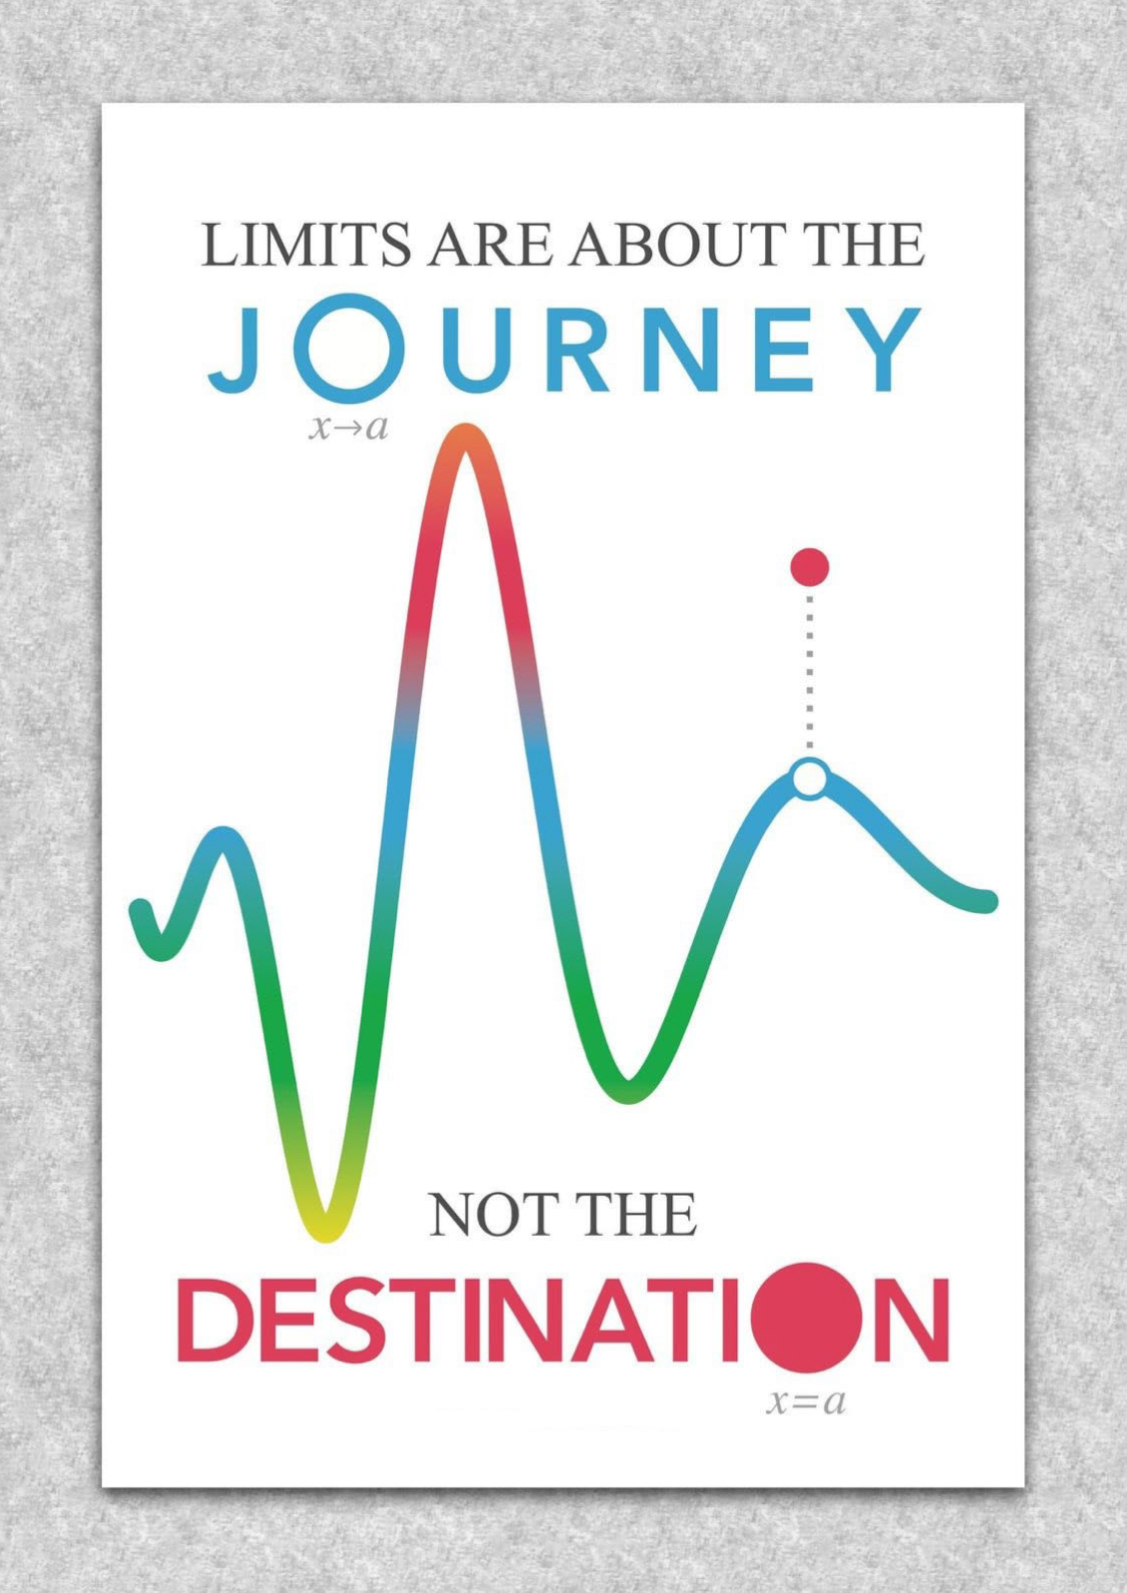
\includegraphics[width=0.2\textwidth]{images/journey.jpg}
	\end{figure}

\item Know that $\ds\lim_{x \to a} f(x)$ exists if and only if $\ds\lim_{x \to a^-} f(x)$ exists, $\ds\lim_{x \to a^+} f(x)$ exits, and $\ds\lim_{x \to a^-} f(x)= \lim_{x \to a^+} f(x)$. 

\item Know the definition and intuitive definition of a limit at $\pm \infty$, e.g. we say that $\ds\lim_{x \to \infty} f(x)= L$ if the outputs of $f(x)$ arbitrarily `close' to $L$ as $x$ gets `larger and larger'.

\item Be able to compute limits at infinity, i.e. $\ds\lim_{x \to \infty} f(x)$ and $\ds\lim_{x \to -\infty} f(x)$, graphically. 

\item Be able to define what a horizontal asymptote and a vertical asymptote is: a horizontal asymptote for $f(x)$ is a line $y= A$ such that $\ds\lim_{x \to \infty} f(x)= A$ or $\ds\lim_{x \to -\infty} f(x)= A$, and a vertical asymptote for $f(x)$ is a line $x= A$ such that $\ds\lim_{x \to A^-} f(x)= \pm \infty$ or $\ds\lim_{x \to A^+} f(x)= \pm\infty$. 

\item Be able to find and identify horizontal asymptotes and vertical asymptotes for a function graphically. 

\item Be able to find and identify horizontal asymptotes and vertical asymptotes for a function algebraically.

\item Understand and be able to use all the limit theorems: if $\lim f= L$ and $\lim g= M$ (and $L, M$ are finite) and $c$ is a real number, then\dots
	\begin{itemize}
	\item $\lim (cf)= c \lim f= cL$
	\item $\lim (f \pm g)= \lim f \pm \lim g= L \pm M$
	\item $\lim (fg)= \lim f \cdot \lim g= LM$
	\item $\lim \left( \tfrac{f}{g} \right)= \tfrac{\lim f}{\lim g}= \tfrac{L}{M}$, if $M \neq 0$
	\end{itemize}

\item (Optional) Know and be able to explain the $\epsilon$-$\delta$ definition of a limit: the limit of $f(x)$ as $x$ approaches $a$ is $L$, denoted $\ds\lim_{x \to a} f(x)= L$, if for all $\epsilon > 0$, there exists $\delta > 0$ such that $|f(x) - L| < \epsilon$ whenever $|x - a| < \delta$. 
\end{itemize}

\end{document}